\documentclass[10pt,conference]{IEEEtran}
\IEEEoverridecommandlockouts
% The preceding line is only needed to identify funding in the first footnote. If that is unneeded, please comment it out.
\usepackage{cite}
\usepackage{amsmath,amssymb,amsfonts}
\usepackage{algorithmic}
\usepackage{graphicx}
\usepackage{textcomp}
\usepackage{xcolor}
\usepackage{enumitem}
\usepackage{siunitx}
\usepackage{listings}
\def\BibTeX{{\rm B\kern-.05em{\sc i\kern-.025em b}\kern-.08em
    T\kern-.1667em\lower.7ex\hbox{E}\kern-.125emX}}
\begin{document}

\title{Novel Assistive Systems Applying Machine Vision and Human-Machine Interaction Technologies for Vulnerable Populations}

\author{
    \IEEEauthorblockN{Y3890959}
    \IEEEauthorblockA{\textit{School of Physics, Engineering and Technology} \\
    \textit{University of York}\\
    York, England}
}

\maketitle

\begin{abstract}
    This article investigates machine vision and human-machine interaction technologies to present two novel systems designed to assist vulnerable populations, encompassing older individuals, people with disabilities, and workers in treacherous conditions. A machine vision-based driver assistance system involving lane, driver's eye-gaze and blink tracking introduces an aid for workers in dangerous environments. Embodying human-machine interaction aspects into this system forms a novel design for cost-effective 'railroad-style' autonomous transportation for older or disabled individuals. Discussions include technical analysis, safety and ethics considerations, and the potential impact on user livelihoods.
\end{abstract}

\begin{IEEEkeywords}
component, formatting, style, styling, insert
\end{IEEEkeywords}

\section{Machine vision-based driver assistance system}
To gauge the driver's focus, a simple driver assistance system must track the vehicle's lane position and the driver's eye gaze and blinks. A vehicle's deviation from the centre of the lane, paired with repetitive blinks or an off-centred gaze in the driver's eyes, denotes extended fatigue or distraction of the driver. With the implementation of an alert system, which alerts not only the driver but other road users, this system can help workers in dangerous conditions, such as truck drivers traversing roads with narrow lanes and combatting fatigue. Abstracting into three fundamental mechanisms can drastically help with the development of this assistance system:

\begin{enumerate}[label=\alph*.]
    \item lane detection and tracking: detection of the lanes and calculating the distances from each side to track the average position of the vehicle.
    \item gaze detection and tracking: detecting and tracking the pupils of the driver's eyes to calculate the average time spent looking off-centre.
    \item blink detection and tracking: detection and tracking of blinking eyelids to calculate the average blinks or the average time of closed eyelids over some time.
\end{enumerate}

\subsection{Lane Detection and Tracking}

The lane departure warning system is quite a mature product, first unveiled in 1989 as a concept and working prototype fitted to the Rover SD1, but later debuted in 2000 as a production-ready system for the Mercedes Actros line of commercial trucks \cite{b1}. Given the safety benefits, lane departure systems have become a mandatory feature for all cars in the European Union as of 2022 \cite{b1}\cite{b2}. The most popular method for detecting lanes across the industry is to employ the Canny edge detection algorithm, The Hough Transform, and various principles of camera calibration, perspective transforms, and colour filtering to determine the lane line edges from a live feed \cite{b1}. Three stages contribute to the lane detection system \cite{b3}:

\begin{enumerate}[label=\alph*.]
    \item pre-processing: low-level image processing consisting of an image crop to reduce the region of interest for more efficient computing, grayscale conversion in preparation for Canny edge detection, and noise reduction techniques such as erosion, dilation and image soothing for more accurate detection.
    \item post-processing: implementation of Canny edge detection resides in this stage using the pre-processed frames to detect the discontinuous lane markings, which The Hough Transform connects into a continuous line.
    \item road lane modelling: computation to detect the left and right lane markings will utilise the continuous line output from the post-processing stage, establishing the positions of the lane boundaries to calculate the vehicle positioning within the lane to detect deviation.
\end{enumerate}

The Hough Transform provides a highly efficient method for detecting straight lines in images, even with noise and missing data \cite{b4}. The Hough Transform works by converting the image space into a parameter space called The Hough Space, and through this space, it is possible to detect geometric shapes by identifying patterns \cite{b5}. This ability of The Hough Transform to identify shapes makes it an ideal tool for detecting lane lines for a self-driving car \cite{b6}.

\subsubsection{Prototype for Lane Detection and Tracking}

Extracting individual image frames from a continuous video stream simplifies the logic of this system. The work in \cite{b3} forms a robust starting point for achieving a lane detection system. As the paper states, there is a cropping step in the pre-processing stage to reduce computational overheads by removing unnecessary parts of the input image. A single-channel conversion to grayscaling will reduce image data complexity to enable faster Canny edge detection. Although the mention of a noise reduction step in \cite{b3}, a detailed explanation nor a visual description is present, leading me to believe its exclusion in the proposed system. As the work in \cite{b7} discusses improvements in the Canny edge detection method by pre-processing the image by stretching the image histogram, the inclusion of a histogram equalisation step will occur post-grayscaling in this system. Inspired by the work in \cite{b6}, applying a Gaussian Blur filter ensures the disregard of as many false edges as possible by reducing noise and smoothening the image.

The work in \cite{b3} mentions, "Canny edge detection is implemented in the post-processing stage." But confusingly, later in the paper, a diagrammatical outline shows this step within the 'pre-processing' stage. The Canny edge detection step will occur in the post-processing stage to avoid confusion and enhance stage separation. Despite applying an image crop, the Canny edge detection will still provide results outside the region of interest (ROI). Inspired by the work in \cite{b6}, cropping the Canny output to the triangular ROI will reduce additional computational overheads and improve The Hough Transform step. Finally, in the post-processing stage, The Hough Transform will generate continuous lines representing the lane marking detections, providing a foundation for lane tracking.

Overlaying The Hough Transform results over the image will provide a visualisation of the machine vision-based road lane marking detection helpful in gauging the system performance. Harnessing the fixed perspective characteristic of the system makes it possible to track vehicle lane positioning by measuring the x-axis location of the vertical base of the left/right lane lines. Veering towards the left lane can be denoted by an increase in the x-axis position of the left-hand lane line base, and veering towards the right can be denoted by a decrease in the x-axis position of the right-hand lane line base. Vehicular deviation from a lane is denoted by whether the base position of each lane line exceeds/falls from a fixed threshold x-axis position value. Threshold optimisation must happen before system implementation by accounting for the width of the vehicle and the perspective/positioning of the camera. Tracking the mid-point x-axis position of the automobile over time, normalising the value w.r.t. the lane positions, and then calculating the variance of this data can measure the driver's dispersion within the lane. This result forms the basis of the metric to gauge the driver's fatigue and focus levels, with a higher variance denoting high fatigue or low focus.

\begin{figure}[htbp]
    \centerline{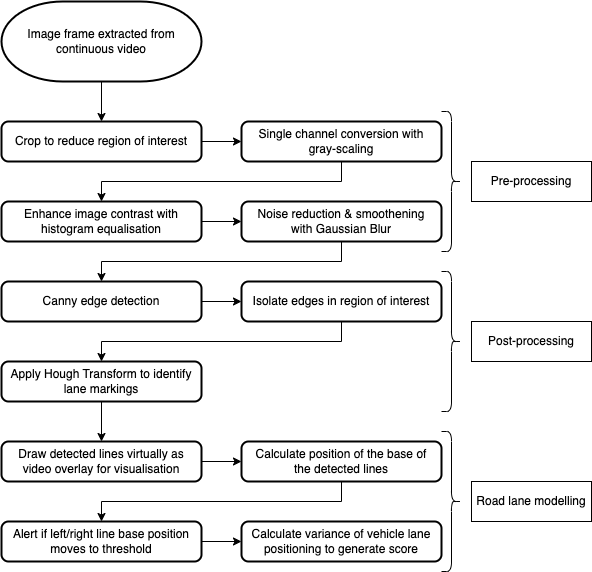
\includegraphics[width=0.5\textwidth]{assets/lane-detection-flow.png}}
    \caption{Flow of lane detection and tracking logic.}
    \label{f1}
\end{figure}

The developed software, source code in Appendix \ref{a1}, utilises the Python programming language and employs the OpenCV library to access highly optimised and efficient computer vision algorithms, reducing development overheads tremendously. The software incorporates a cropping stage before processing the frame to ensure compatibility with a wide range of input video dimensions. A constant definition for the height and width of the input video feed is present, which the initial crop utilises for generating a window aligned at the bottom of the original frame and horizontally centred, ensuring a 640(w)x480(h) crop (dimensions as defined by the constants) for any higher resolution video feed. This cropping is merely for input video dimension standardisation, and regions outside of the ROI will still be present to ensure easy data visualisation. A YouTube video \cite{b8} forms the perfect testing input for this system, consisting of an almost 4-hour video feed of a nighttime drive from Busan to Seoul through various types of roads and lighting conditions.

\begin{figure}[htbp]
    \centerline{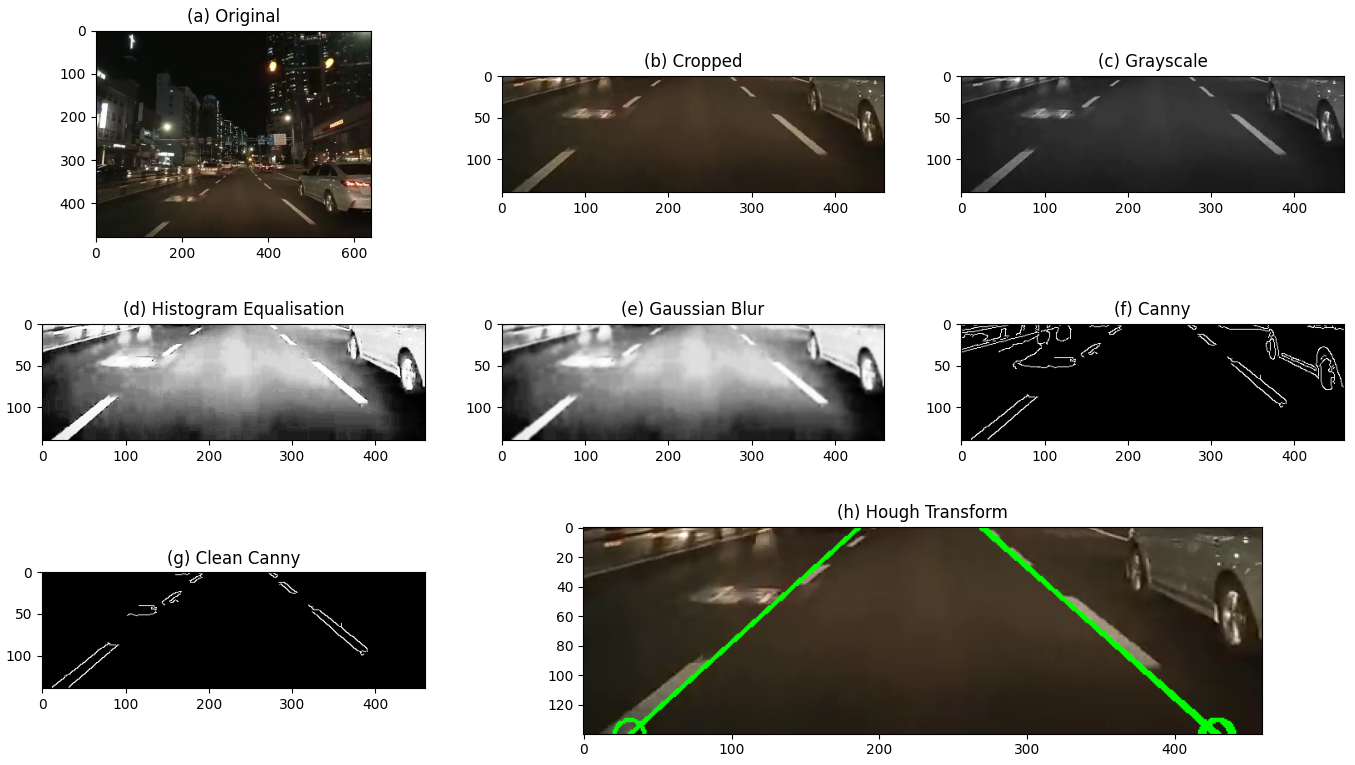
\includegraphics[width=0.5\textwidth]{assets/LDS_plot.png}}
    \caption{Stage-by-stage plots of the lande detection and tracking system outputs. Original frame shown in (a) which is then cropped in (b), grayscaling filter applied in (c), with histogram equalisation in (d) and a Gaussian blur in (e), output from the Canny edge detector in (f), with results cropped and shown in (g), the road lane markings identified by The Hough Transform are overlayed on to the frame in (h).}
    \label{f2}
\end{figure}

After the input video feed standardisation to 640x480, the first step in the pre-processing stage is an additional frame crop to reduce the ROI. Using the matplotlib Python library, a plot of the normalised video with the axis labels can help choose the lane width with the lane markings and how far forward the system needs to see. With the ROI region coded as shown in Figure \ref{f2}, grayscaling occurs to reduce computational complexity by converting to a single-channel image. The application of histogram equalisation, then a Gaussian blue filter, prepares the frame for the post-processing stage of the system.

Implementing a zero-parameter automatic Canny edge detection logic simplifies the system greatly \cite{b9}. Though not truly a 'zero-parameter' due to the necessity of a threshold 'sigma' parameter, it vastly simplifies logic using statistical offsets, enabling single parameter tweaking for optimisation. A further crop with an isosceles trapezoid-shaped masking window on the Canny algorithm output eliminates all edge information outside the lane markings, further isolating the ROI. The clean Canny output enables a more efficiently performed Hough Transform to detect the road lane markings. The Hough Transform implementation has further logic to ensure only lines within a specified diagonal angle range are output from the step to ensure only lane markings are detected. The definition of programmatical constants for the angle range values enables simple optimisation. The Hough Transform generated lines drastically extend the frame size due to the presence of a multiplier as per the OpenCV tutorial documentation \cite{b10}. Modifications to The Hough Transform logic in this lane assist implementation include scaling the detected and drawn lines to fit within the border of the image frame. Programmatical detection of road lane markings consists of parsing the start and end coordinates of the detected lines. The Hough Transform generates two coordinate points for each detected line, with a starting point at the bottom of a positive gradient line and at the top of a negative gradient line. More simply, starting points will be on the left and ending points on the right.

Left-hand lane markings will start at a y-axis value equal to the frame height and finish at a y-axis value equal to 0, with arbitrary x-axis values. Right-hand lane markings begin at the top and end at the bottom of the frame, with arbitrary x-axis values. This understanding makes it easier to differentiate between the two sides of lane markings and to parse the position of the base of each line. The departure warning implementation will use the base positions of each lane marking, alerting once each position passes an x-axis threshold (programmatically defined as a constant). Shown in Figure \ref{f2} is the implementation in action with lane detections shown in green and the bases of each also circled in green. When the driver approaches too closely to either lane, the lines will turn red, alerting a lane departure. The vehicle lane tracking implementation collects the base location of left-hand and right-hand lane markings, using linear interpolation for intermediate predictions for frames with undetected lane markings. The centre point between the two lane markings is the vehicle's position. Calculating the driver's lane position variance (LPV) metric, showing the variance in the vehicle's position w.r.t. the lane markings, is possible using an array of vehicle positions. Including garbage collection to limit the maximum and minimum number of collected vehicle position data by deleting old data once passing the maximum threshold prevents a gradual slow-down of the program due to a massively growing array.

\begin{figure}[htbp]
    \centerline{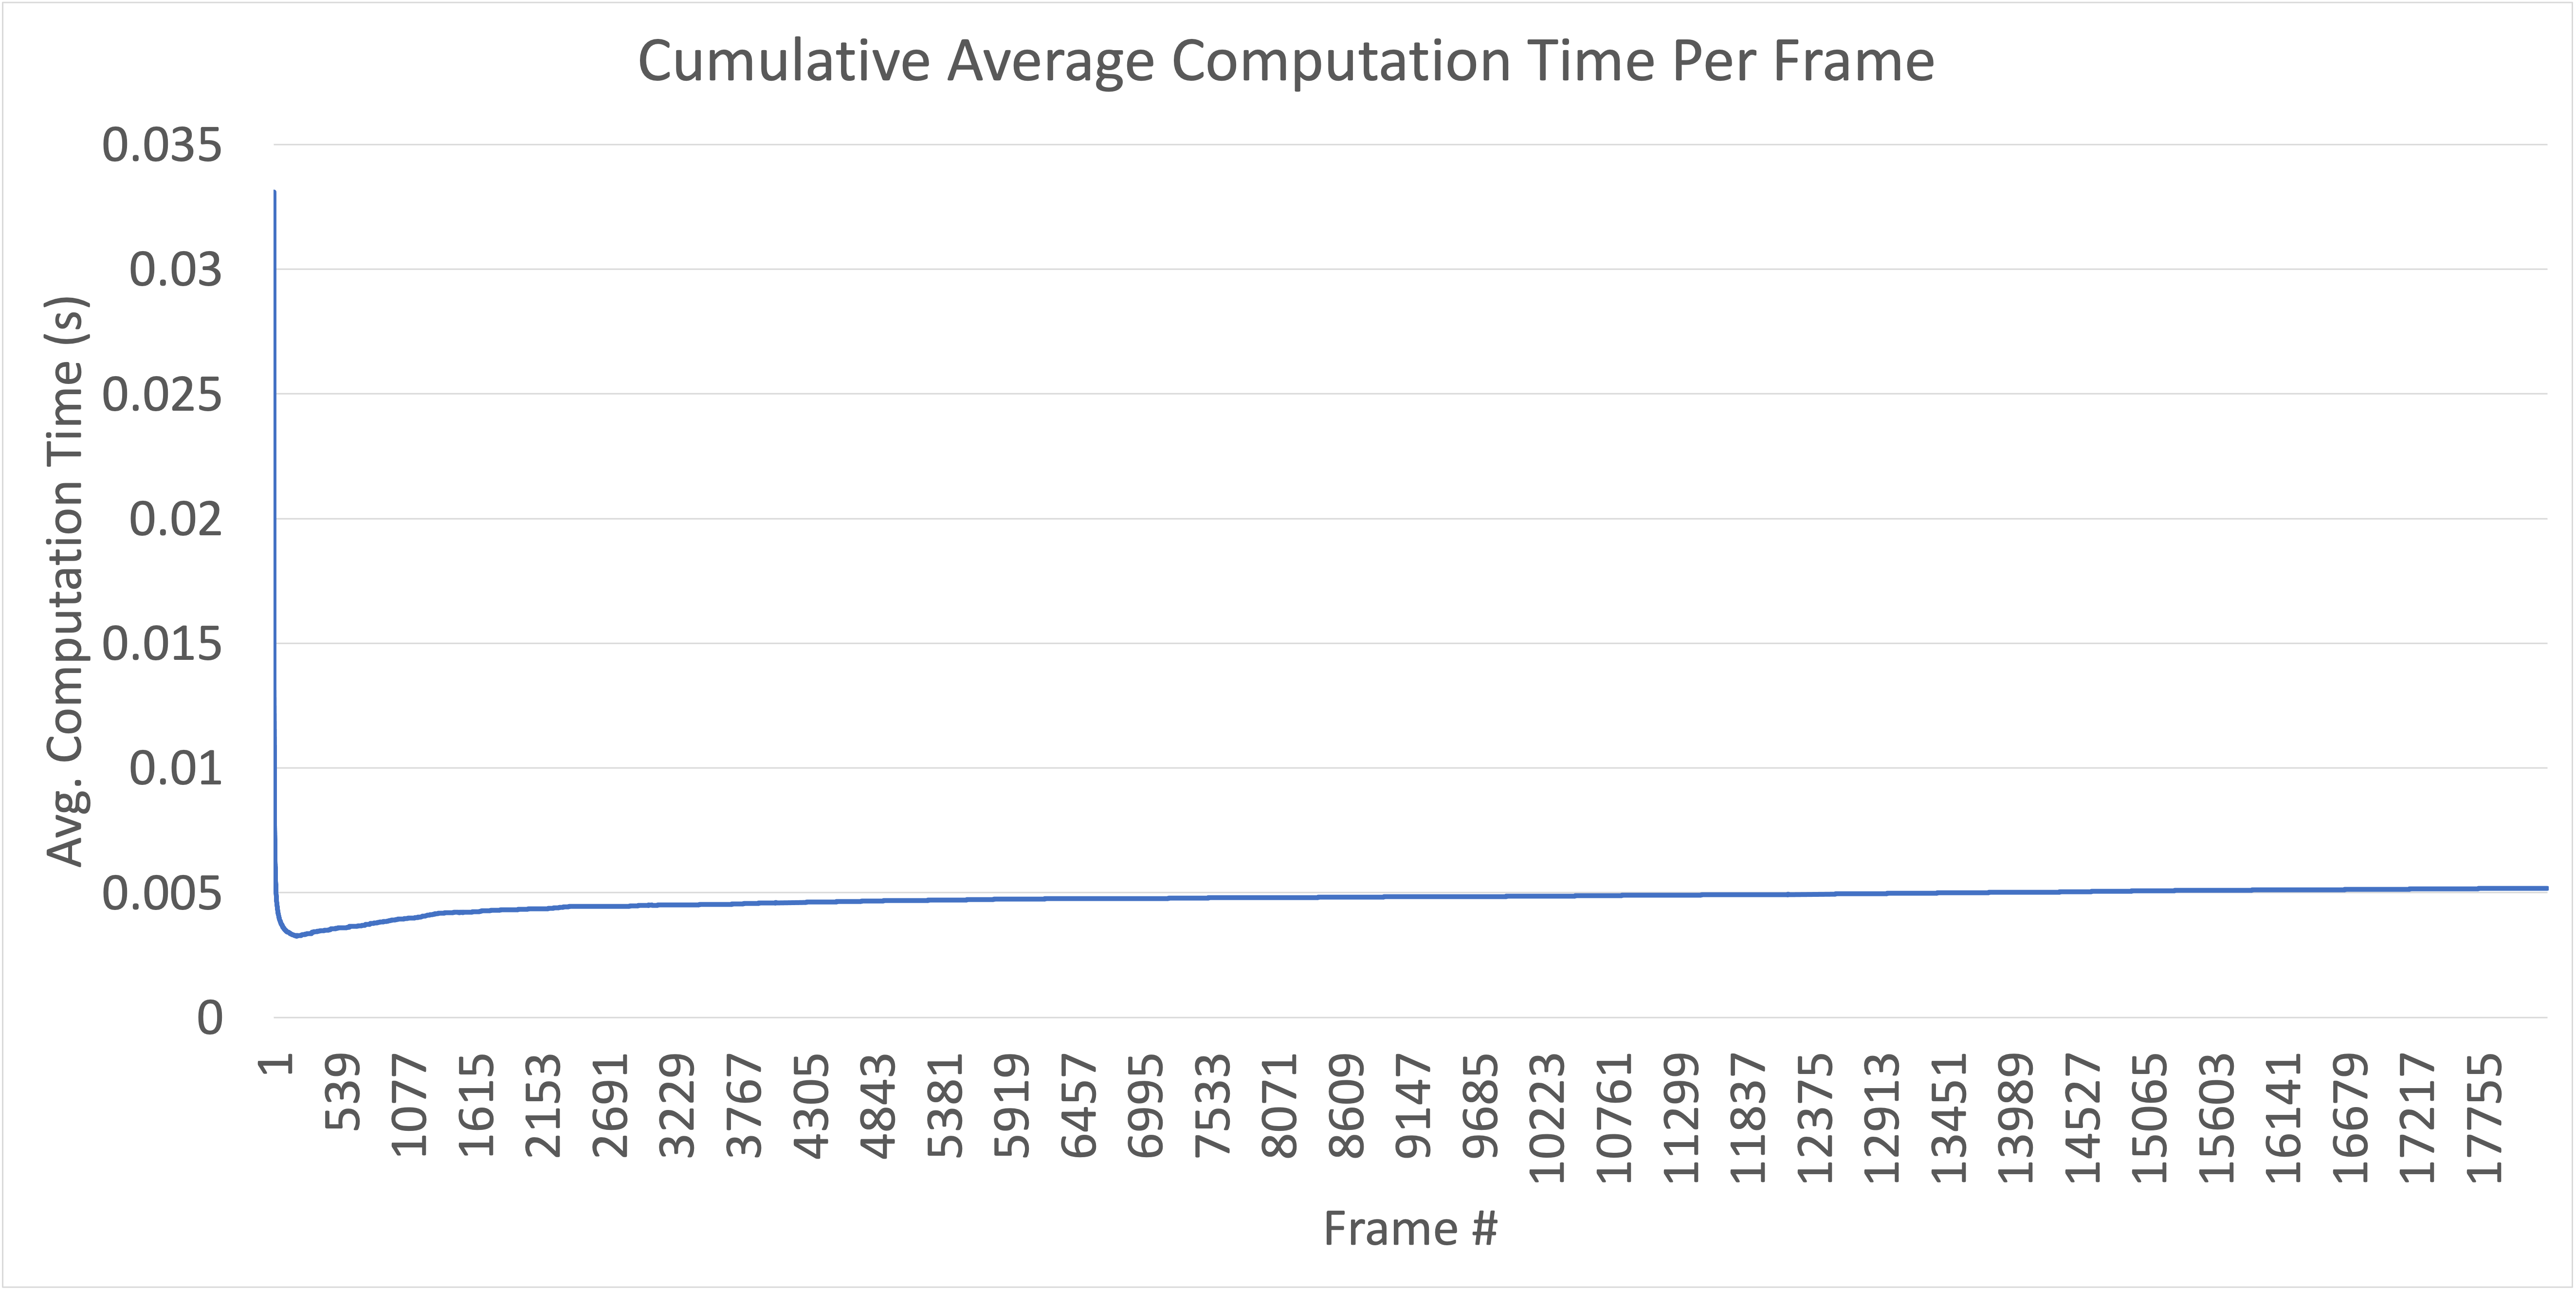
\includegraphics[width=0.5\textwidth]{assets/LD_Avg-FPT.png}}
    \caption{Cumulative average of the time taken to compute each frame for lane detection and tracking.}
    \label{f3}
\end{figure}

\begin{figure}[htbp]
    \centerline{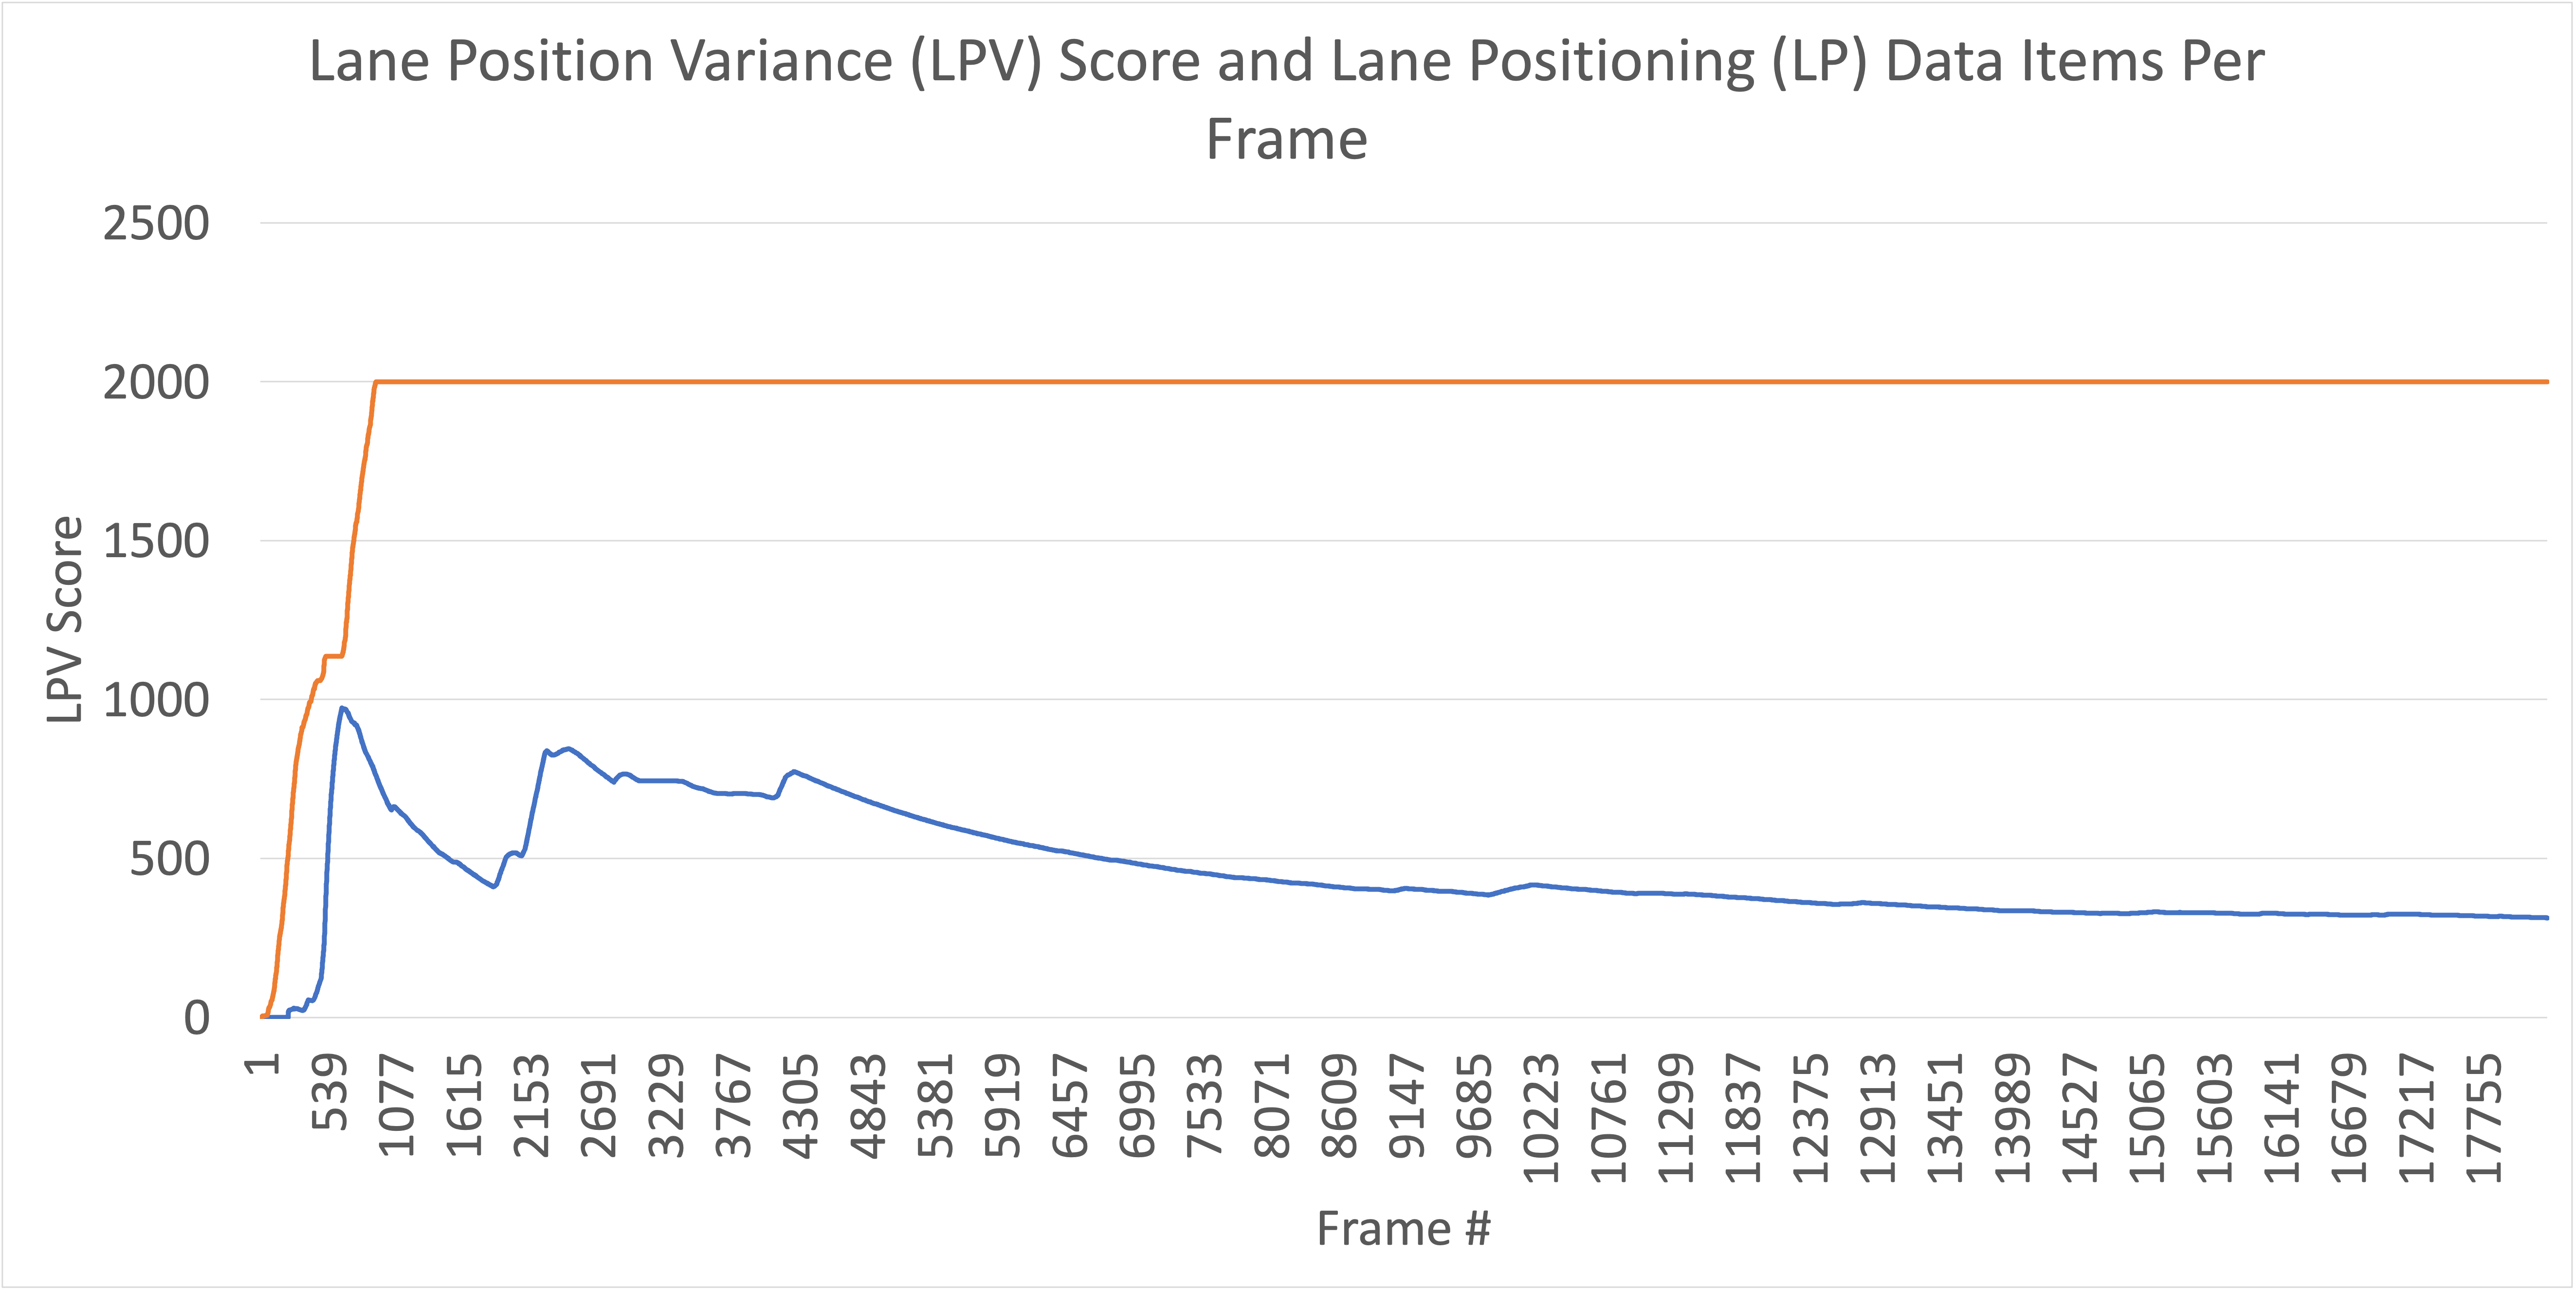
\includegraphics[width=0.5\textwidth]{assets/LD_Avg-LPV.png}}
    \caption{(Blue trace) cumulative average of the LPV score at each frame for lane detection and tracking, calculated using the footage between 0:18-13:00 from the testing video \cite{b8}. (Orange trace) number of lane positioning data items used to compute LPV score.}
    \label{f4}
\end{figure}

The mission-critical essence of this system permeates from its fundamental requirement of detecting and alerting hazards as they occur. The processing time for each frame must be as low as possible to ensure the software can keep up with the input video feed. The system implements start and finish timestamping to acquire metrics for real-time performance. The YouTube video as before \cite{b8} but only including the footage between 0:18 and 13:00 forms the basis of these real-time metrics plots in Figure \ref{f3} and Figure \ref{f4}. Shown in Figure \ref{f3} is the cumulative average for the time taken to compute each frame. We can see an average frame compute time of \SI{5.2}{\micro\second}, resulting in an average of roughly 192 frames per second. It is unclear what caused the tremendous spike in compute time during the first frame, but I assume this to be OpenCV-related, resulting from populating GUI windows for the first time.

Shown in Figure \ref{f4} is a plot of the lane position variance, a score calculated from the cumulative average of the variance in the vehicle's position w.r.t. the lane markings from each frame. The spikes in this score at the beginning of the footage are due to the driver making multiple lane changes and swaying within the lane. However, once the driver enters the motorway, the score starts to settle down, a result of fewer to no lane changes and swaying. The graph also has an overlayed plot of the number of lane positioning data items, a count of the total number of left-hand and right-hand lane base positions. To ensure as much interpolation accuracy as possible, the calculation of the LPV score only starts when there is a minimum of 500 previously recorded lane marking positions. The higher the amount of lane position data points, the slower the linear interpolation algorithm will be. The system's effort to maintain a maximum of 2000 points to ensure performance is visible as the graph plateaus at this value.

\subsection{Blink and Gaze Detection and Tracking}

Although separating blink and gaze aspects into individual blocks helps with conceptualising the system, in implementation, it is much easier and more efficient to merge them into a single block. The first driver monitoring implementation was introduced by Toyota in 2006 for its and Lexus' latest models, incorporating face tracking using IR LED detectors and CCD cameras \cite{b11}. Although 18 years have passed since then, only a handful of car manufacturers have adopted this technology, including BMW, Ford, Cadillac, NIO, XPeng, and Mercedes-Benz, incorporating this technology in some of their models. Albeit regulated, this technology is not yet mandatory as per the European Union \cite{b12}, which could be the primary cause for this lacklustre adoption. As a result, there is no industry-standard methodology for this system. This system follows the same three-stage abstraction as the lane detection and tracking flow. The pre-processing stage is identical. The post-processing now includes Dlib machine learning-based functions \cite{b13} to detect faces and predict facial landmark coordinates, utilising Dlib's pre-trained 68-point facial model \cite{b14}. Finally, a binary inversion threshold filter before a Simple Blob Detection step facilitates pupil/iris detection. The final stage consists of driver monitoring logic, where results computation from the pre and post-processing stages occur to calculate the driver's fatigue and focus levels.

\begin{figure}[htbp]
    \centerline{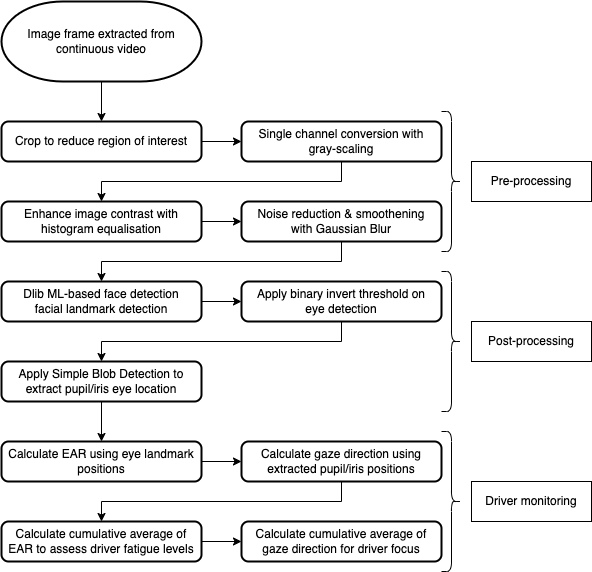
\includegraphics[width=0.5\textwidth]{assets/eye-detection-flow.png}}
    \caption{Flow of eye blink and gaze detection and tracking logic.}
    \label{f5}
\end{figure}

\subsubsection{Prototype for Gaze and Blink Detection and Tracking}

Following a similar approach to \cite{b15}, the programmatical implementation for this system, source code in Appendix \ref{a2}, uses a similar logic from the lane detection and tracking implementation. A crop is present to reduce the resolution of the feed to 640x480, programmatically defined as a constant, to speed up frame processing time. Grayscaling, histogram equalising and Gaussian filtering steps are present to improve system efficiency for detection and processing time, in addition to drastically enhancing the low light capabilities of this system. The detection of faces and facial landmarks is possible using the Dlib detection function with the trained 68-point landmark model. The eye aspect ratio (EAR) enables the detection of blinks by deriving from the positions of detected eye landmarks using the dimensions of the left and right eyes. The system calculates a cumulative average EAR over a fixed amount of time to form the driver tiredness score, currently set to a 600 frame sample size, which equates to 10 minutes for a 30 FPS input. The implementation alerts if the tiredness score drops below a certain threshold, notifying the driver that most of the 10-minute sample size consists of shut or near-shut eyelids.

Isolating each eye as a window is possible since landmarking accurately identifies each eye's coordinate bounds. With each isolated eye, applying a binary threshold allows for a clear separation between the pupils/iris and the sclera, forming an ideal preparation for the OpenCV Simple Blob Detection algorithm \cite{b16}. The initialisation of the Simple Blob Detector consists of deactivating the thresholding stage since the implementation already grayscales the frame. Filtering by colour is enabled, correctly setting the thresholded colour of the pupils/iris. Filtering by area is enabled since testing revealed that the dark spots of the pupils/iris take up most of the space in the frame.

\begin{figure}[htbp]
    \centerline{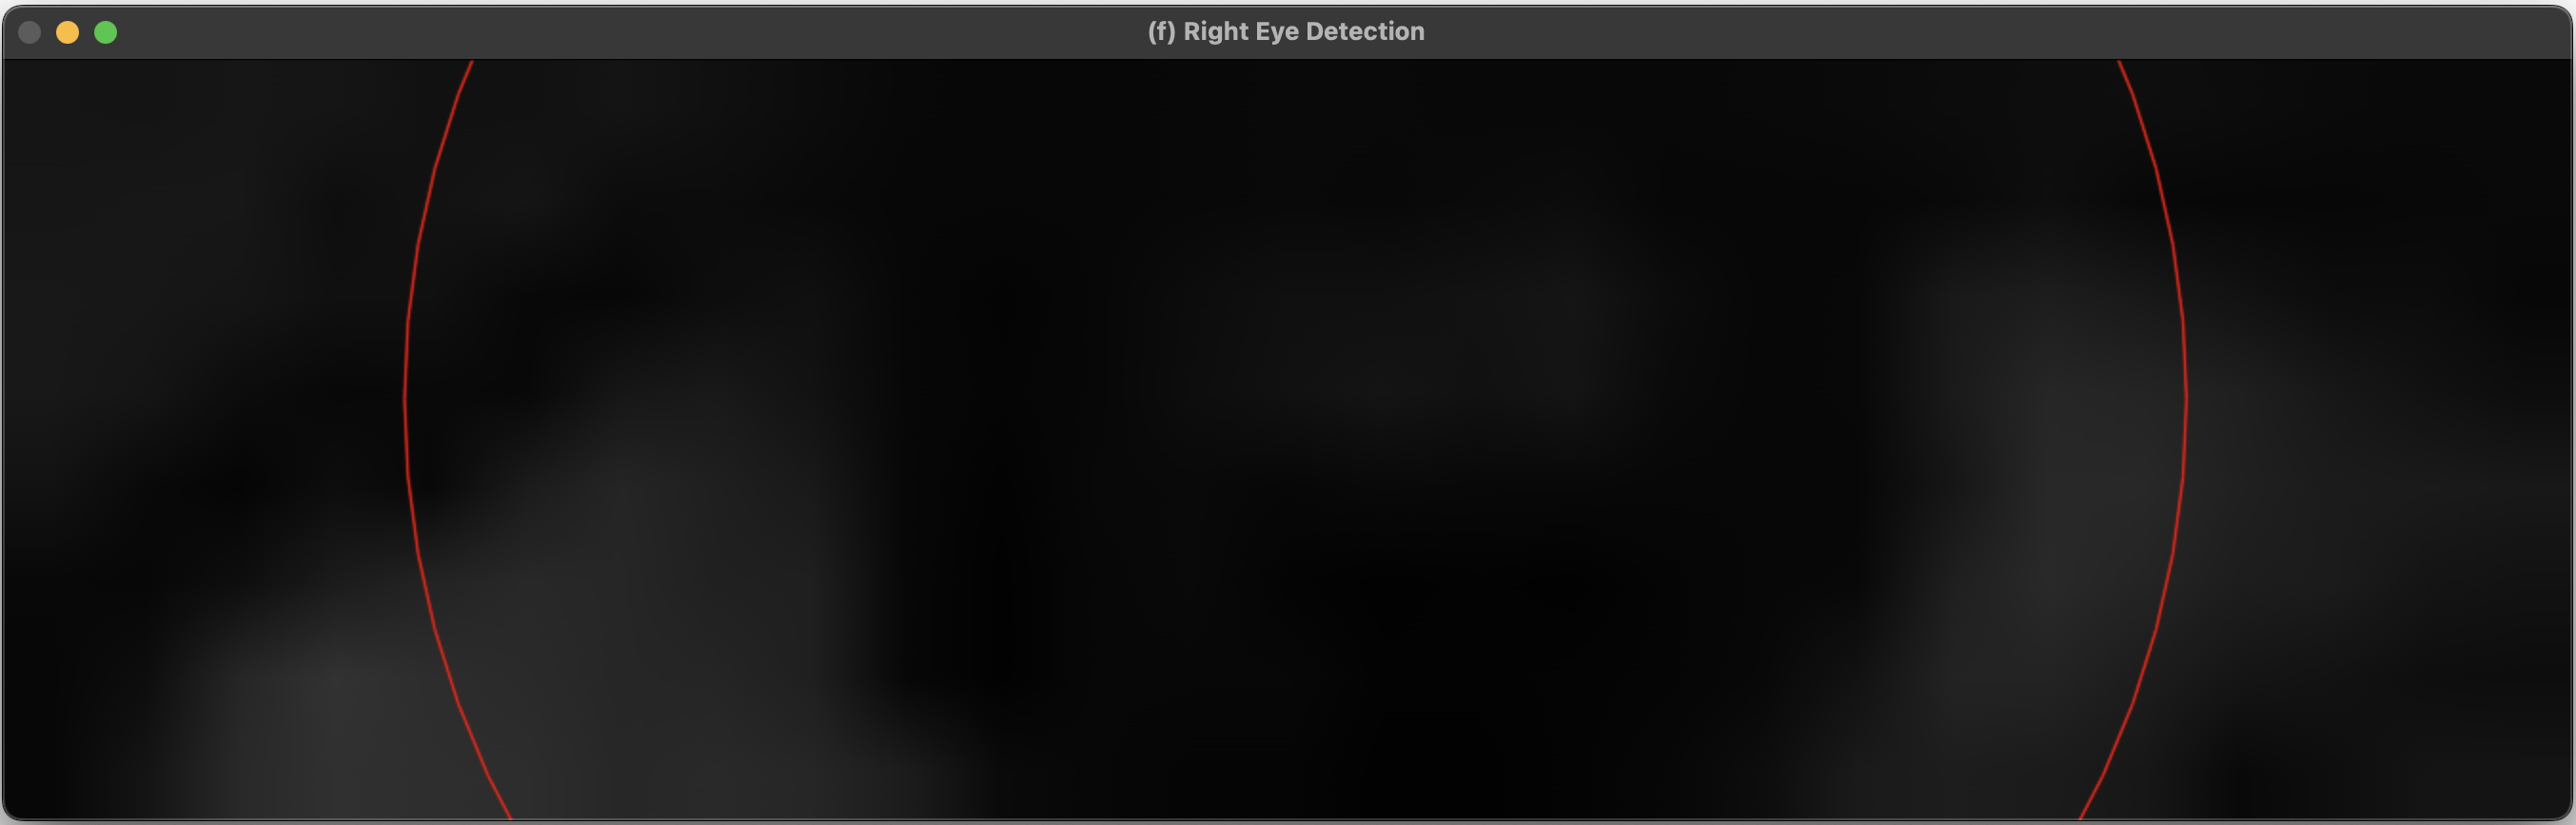
\includegraphics[width=0.5\textwidth]{assets/gaze-detection.png}}
    \caption{Visualisation of pupil/iris detection using the Simple Blob Detector for the gaze tracking system.}
    \label{f6}
\end{figure}

\begin{figure}[htbp]
    \centerline{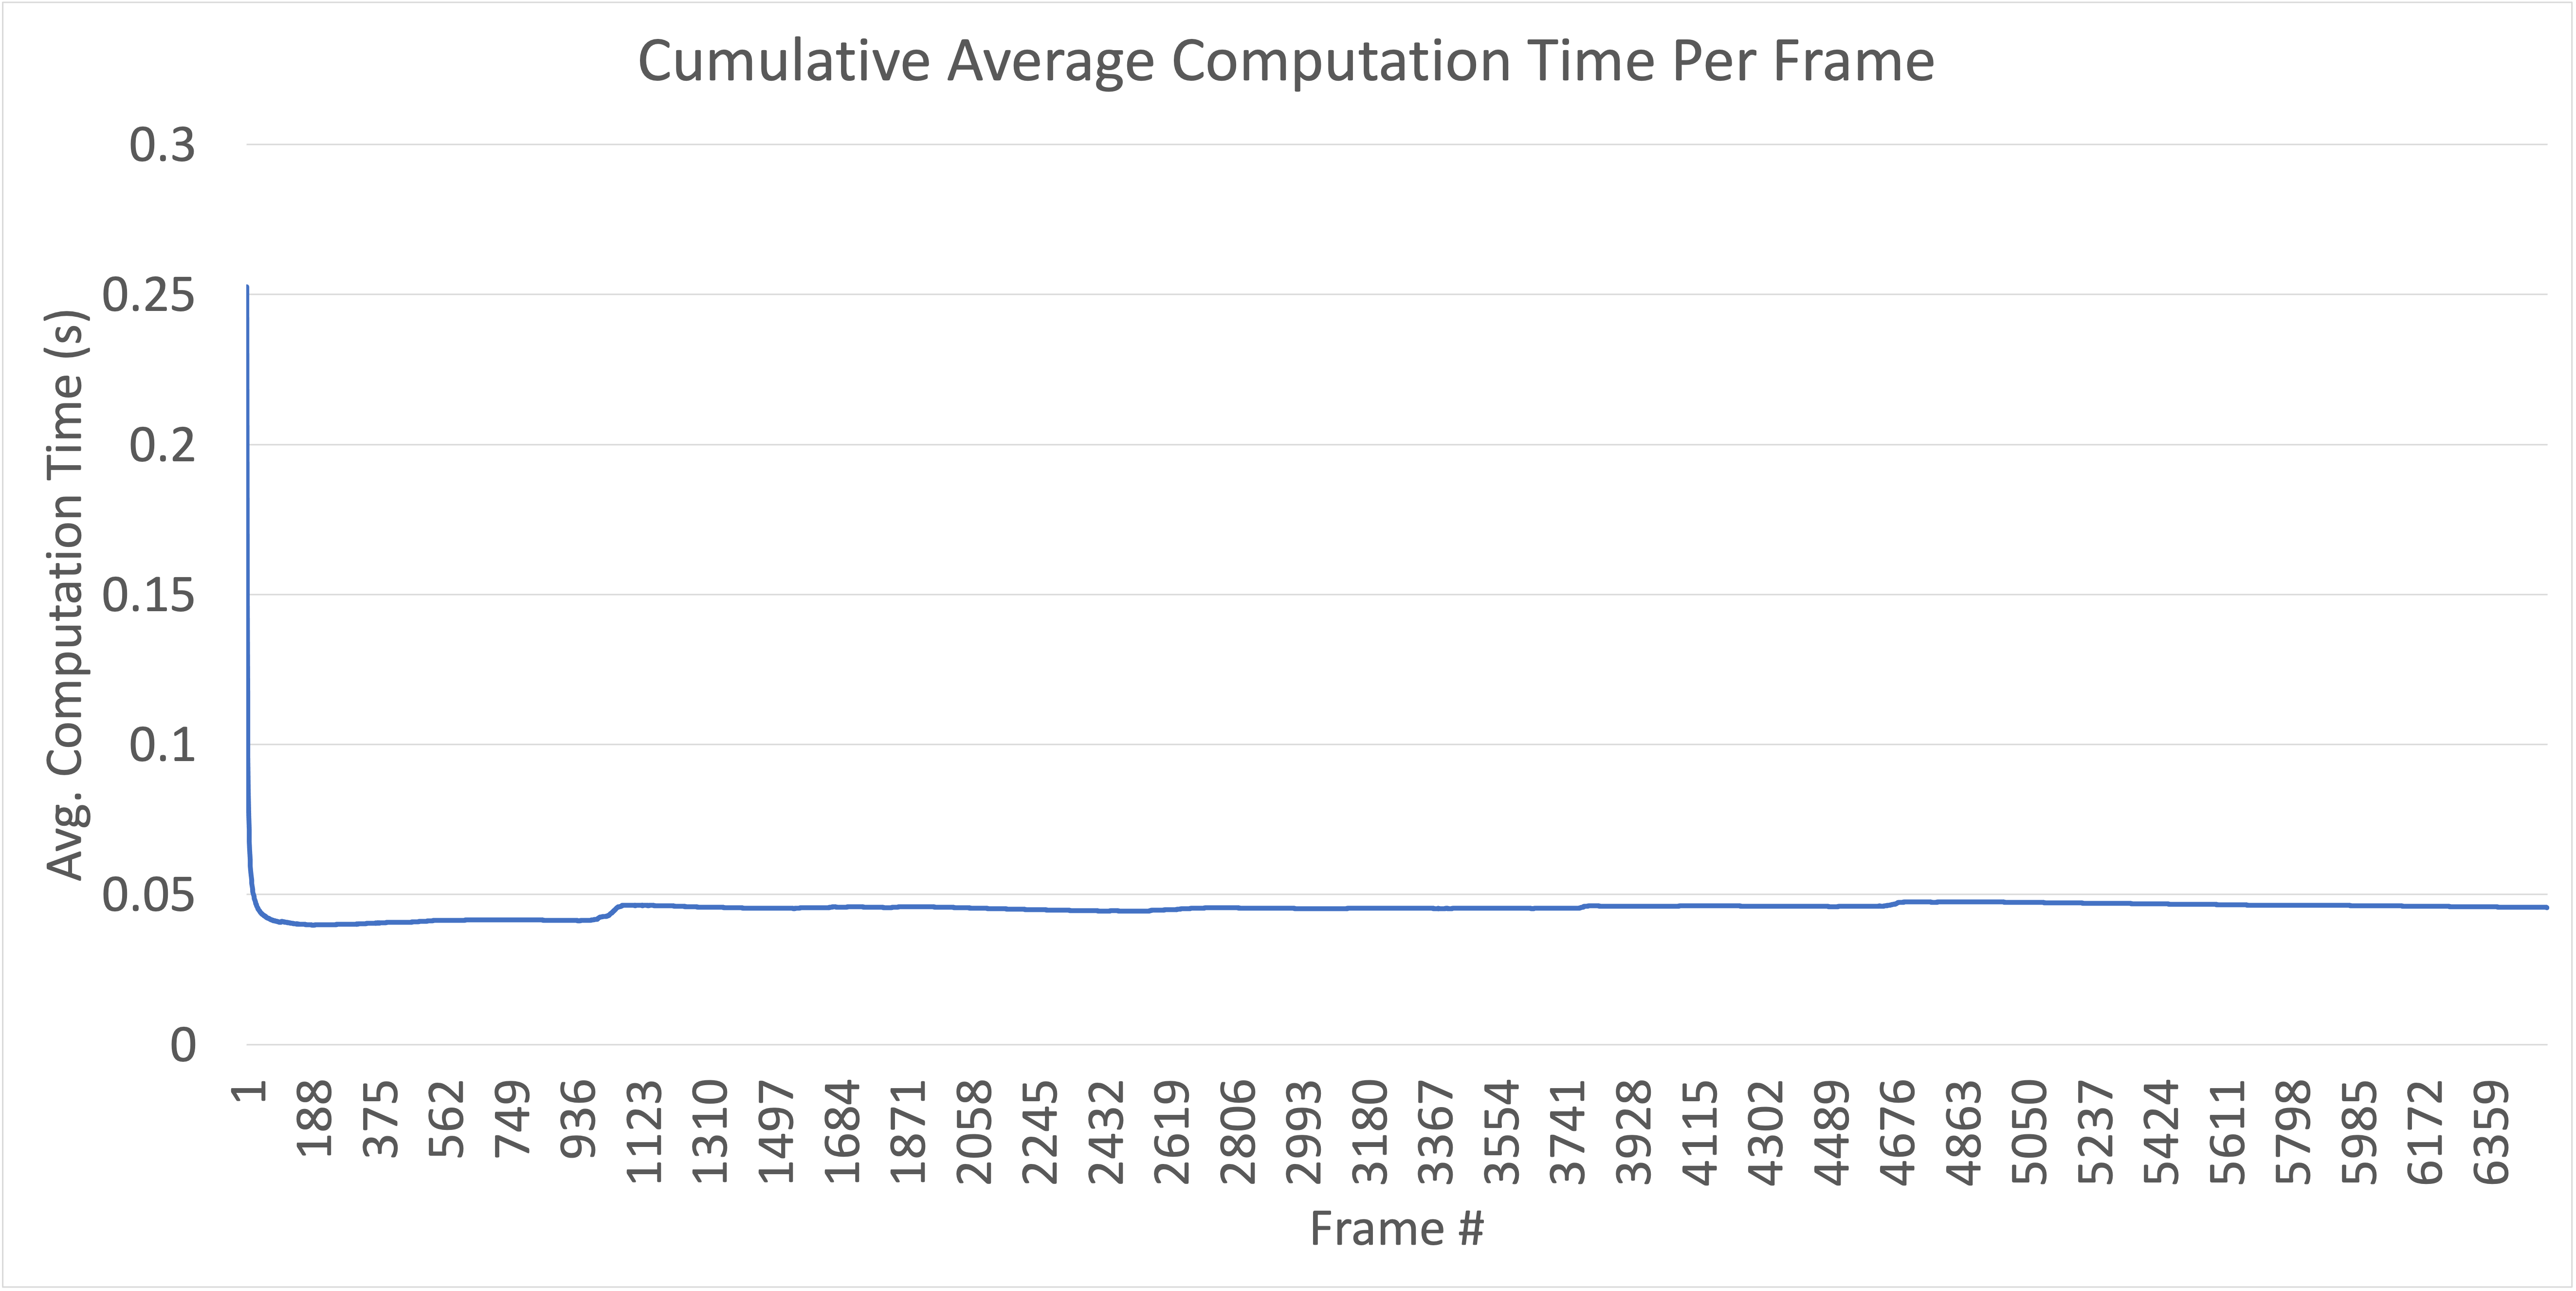
\includegraphics[width=0.5\textwidth]{assets/Eye_Avg-FPT.png}}
    \caption{Cumulative average of the time taken to compute each frame for eye detection and tracking.}
    \label{f7}
\end{figure}

Figure \ref{f6} shows the result of the blob detection, detecting the iris successfully. Though quite reliable at tracking left and right gaze directions, a paramount downside is that it does not track up and down movements competently, as the blob detection fails to detect. Tracking all gaze locations is crucial for a driver monitoring system. Workarounds are present, such as measuring the time the driver spends looking straight, left, or right since tracking this is comparatively reliable, then inverting this to generate the time the driver spends not looking ahead, allowing a gauge on the driver's focus. Despite lacking gaze tracking functionality, Figure \ref{f7} shows an average \SI{45}{\micro\second} frame compute time, with the same spike in the first frame, just like the lane detection and tracking system. The average frame compute time value exhibits an approximate 25 frames per second compute rate for this system, only a five frames per second difference from my webcam capture rate.

\begin{figure}[htbp]
    \centerline{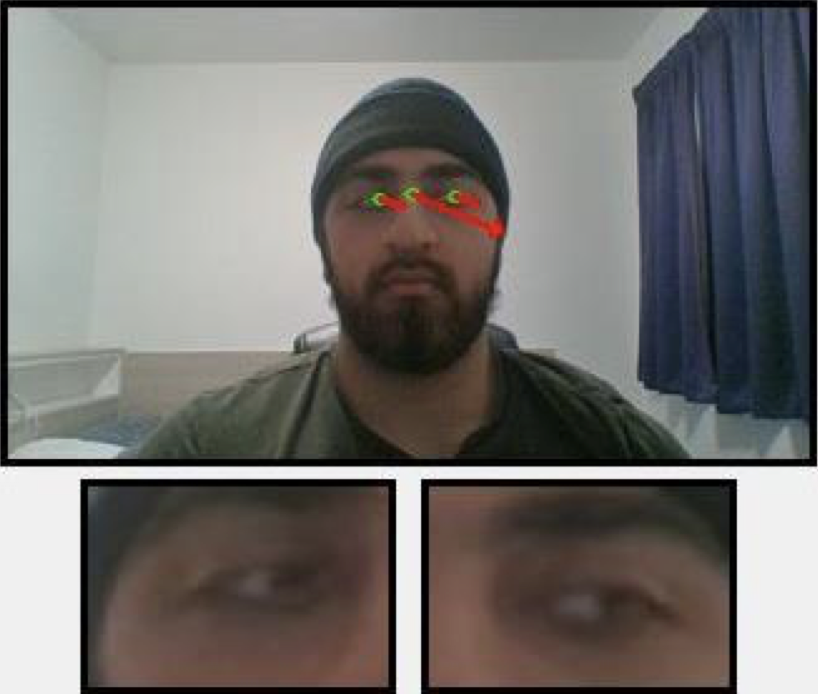
\includegraphics[width=0.5\textwidth]{assets/Gagan-eye.png}}
    \caption{Eye gaze and blink tracking demonstration of a different system [18].}
    \label{f8}
\end{figure}

Unlike the lane detection and tracking system, a highly efficient frame computing capability is not a necessity for this system. Due to its reduced mission criticality, the fundamental goal would instead be to focus on highly accurate gaze tracking. The work in \cite{b17} implements a Regression Convolutional Neural Network on top of the facial landmark detection to track eye gaze. Initialising and running the Python code associated with this paper, located in a GitHub repository \cite{b18}, reveals a veraciously impeccable gaze detection implementation achieved by accelerating traditional machine-vision methodologies using machine-learning techniques, shown in Figure \ref{f8}. The improved tracking accuracy comes at a price of performance, but this substantial drop in frame rates is a sacrifice to gain reliable measurements.

\subsection{Implementation of System}

Interlinking the lane detection and tracking system with the blink and gaze detection and tracking implementation assembles the complete driver assistance solution. Computing an overall score using the LPV and tiredness/focus score from the two individual systems is possible and can gauge the driving safety score for the driver. The prospect of employing several interaction modalities can improve the safety of the driver and surrounding traffic:

\begin{enumerate}[label=\alph*.]
    \item Visual feedback: A visualisation of the detected lane markings coloured to portray lane departure can be overlayed on a video feed, perhaps augmented via a heads-up display, providing assistance to maintain centred lane positioning. Alerts to show in the instrument cluster or heads-up display when the driver struggles to maintain centre position (LPV score above threshold), when the driver's blinking is more frequent (tiredness score via blink tracking above threshold), or when the driver's focus is low (focus score via gaze tracking below threshold). External car lighting can alert the driver and surrounding traffic by implementing a similar design as Audi \cite{b19} by integrating results from this driver assistance system. Matrix LED headlight technology draws symbols on the road to emphasise lane markings, with warning triangles and concentrated light flashes to warn the driver and surrounding traffic and organic LED taillights to provide visual information to surrounding traffic.
    \item Auditory feedback: Employing spacial audio cues for lane departure warnings, developed in a way where the audio direction comes from the side of the lane departure, forms the ultimate warning system. It's not necessarily noise that keeps you awake - it's the sudden change in noise that's most likely to wake you up \cite{b20}. Harnessing this ideology can administer a prime solution to combat driver fatigue; playing a loud sporadic noise, such as a dog barking at random intervals when the tiredness score surpasses a certain threshold, can help wake the driver. A more ordinary solution is to display an alert on the instrument cluster or a heads-up display to suggest the driver take a coffee break.
    \item Haptic feedback: Vibrations or physical movements of the steering wheel can alert the driver of lane departure. Since the system knows the lane positioning, it can take a further step by applying steering inputs to ensure the vehicle maintains a centred position within the lane. Implementation of seat vibrations can enhance the alert system, especially in the case where the driver is asleep or unconscious with both hands off the steering wheel. A more aggressive seat jolt, implemented in the same fashion as the load sporadic dog barking, can wake the driver more efficiently.
    \item Climatory feedback: Upon driver fatigue detection, the driver assistance system can autonomously set the car's climate to an unbearably cold cabin temperature, catalysing an unpleasant thermal environment to wake the driver. Some car manufacturers, such as BMW \cite{b21}, have implemented climate-control-based cabin scent diffusers, crafting a perfect method to wake the driver when fatigued by filling the cabin with citrus, coffee, or similar aromatherapeutic scents to stimulate the brain \cite{b22}.
\end{enumerate}


\subsection{Safety, Ethics, and Impact of System}

Statistics show that a lane assist system results in an 11\% reduction in crashes of all severities and a 21\% reduction in crashes with injuries, with results suggesting the saving of thousands of lives each year if every passenger vehicle in the US implements a lane departure warning system \cite{b23}. Studies show that human error, including fatigue or drowsiness, contributes to 80.6\% of road accidents \cite{b24}, with reports stating that 54\% of adult drivers feel drowsy while driving and 28\% attesting that they fall asleep while driving \cite{b25}, the need for a reliable driver fatigue detection and monitoring system, which alerts the driver has never been more imperative as our reliance on vehicles has exponentially increased, leading to higher levels of road users.

Despite the high praise for driver assistance technologies, a voluminous risk still exists involving the shift of trust to machine vision and computer algorithms to perform safety-critical decisions. For example, false lane detection alerts can potentially startle the driver and lead them to perform unsafe manoeuvres to mitigate a risk that was never present. Moreover, the driver monitoring system responsible for tracking driver docus and fatigue, when implemented into driving trackers (black-box trackers) for car insurance policies, can result in adverse insurance premium changes due to false results. Strategies to improve system performance for enhanced environment tracking are present, though a computer vision approach can never be perfect due to varying environmental conditions. A key factor to mitigate the risk is considering these systems as a helping hand and not holding predominant trust in them. Another aspect to consider is privacy and ethicality, especially with the constant recording of surrounding roads and the driver's face to ensure system functionality. Employment of edge computing, ensuring all data processing occurs within the vehicle, can mitigate privacy risks by preventing data transfer to servers. However, this can drastically bottleneck the system performance as power-limited and smaller form factor computers inside vehicles replace the powerful and centralised server farms.

70\% of survey respondents believe that in-vehicle Driver Monitoring Systems can improve road safety and help reduce accidents caused by distracted or fatigued drivers, with only 28\% of UK consumers knowing this new technology \cite{b26}. Carmakers and regulators must strive for widespread adoption, to raise awareness, and to improve road safety for all.

\begin{thebibliography}{00}

    \bibitem{b1} "Lane departure warning system," Wikipedia, https://en.wikipedia.org/wiki/Lane\_departure\_warning\_system (accessed Dec. 27, 2023).

    \bibitem{b2} "Press corner," European Commission - European Commission, https://ec.europa.eu/commission/presscorner/detail/en/ip\_22\_4312 (accessed Dec. 27, 2023).

    \bibitem{b3} C. Y. Low, H. Zamzuri and S. A. Mazlan, "Simple robust road lane detection algorithm," 2014 5th International Conference on Intelligent and Advanced Systems (ICIAS), Kuala Lumpur, Malaysia, 2014, pp. 1-4, doi: 10.1109/ICIAS.2014.6869550.

    \bibitem{b4} L. Chandrasekar and G. Durga, "Implementation of Hough Transform for image processing applications," 2014 International Conference on Communication and Signal Processing, Melmaruvathur, India, 2014, pp. 843-847, doi: 10.1109/ICCSP.2014.6949962.

    \bibitem{b5} A. R, “Hough transforms in image processing,” Scaler Topics, https://www.scaler.com/topics/hough-transform-in-image-processing/ (accessed Dec. 28, 2023).

    \bibitem{b6} N. Vykari, “Understanding Hough Transform with a lane detection model,” Paperspace Blog, https://blog.paperspace.com/understanding-hough-transform-lane-detection/ (accessed Dec. 28, 2023).

    \bibitem{b7} T. Tasneem and Z. Afroze, "A New Method of Improving Performance of Canny Edge Detection," 2019 2nd International Conference on Innovation in Engineering and Technology (ICIET), Dhaka, Bangladesh, 2019, pp. 1-5, doi: 10.1109/ICIET48527.2019.9290676.

    \bibitem{b8} RideScapes, “ASMR highway driving at night (no talking, no music) - busan to Seoul, Korea,” YouTube, https://www.youtube.com/watch?v=nABR88G\_2cE (accessed Dec. 30, 2023).

    \bibitem{b9} A. Rosebrock, “Zero-parameter, automatic canny edge detection with python and opencv,” PyImageSearch, https://pyimagesearch.com/2015/04/06/zero-parameter-automatic-canny-edge-detection-with-python-and-opencv/ (accessed Dec. 30, 2023).

    \bibitem{b10} “Hough Line transform,” OpenCV, https://docs.opencv.org/3.4/d9/db0/tutorial\_hough\_lines.html (accessed Dec. 30, 2023).

    \bibitem{b11} “Driver monitoring system,” Wikipedia, https://en.wikipedia.org/wiki/Driver\_monitoring\_system (accessed Jan. 3, 2024).

    \bibitem{b12} Council of European Union, Council regulation ({EU}) no 2019/2144, https://eur-lex.europa.eu/eli/reg/2019/2144/oj (accessed Jan. 3, 2024).

    \bibitem{b13} “Classes,” Dlib C++ Library, http://dlib.net/python/index.html (accessed Jan. 3, 2024).

    \bibitem{b14} “Trained 68-Point Facial Landmark Model,” Dlib C++ Library, http://dlib.net/files/shape\_predictor\_68\_face\_landmarks.dat.bz2 (accessed Jan. 3, 2024).

    \bibitem{b15} B. Yagyesh, “Eye blink detection with opencv, python, and dlib,” GeeksforGeeks, https://www.geeksforgeeks.org/eye-blink-detection-with-opencv-python-and-dlib/ (accessed Jan. 3, 2024).

    \bibitem{b16} “CV::Simpleblobdetector class reference,” OpenCV, https://docs.opencv.org/3.4/d0/d7a/classcv\_1\_1SimpleBlobDetector.html (accessed Jan. 3, 2024).

    \bibitem{b17} G. Malhotra, “Building a Prototype to Track Eye Gaze,” dissertation, 2023

    \bibitem{b18} G. Malhotra, “GagandeepMalhotra/Building-a-Prototype-to-Track-Eye-Gaze,” GitHub, https://github.com/GagandeepMalhotra/Building-a-Prototype-to-Track-Eye-Gaze (accessed Jan. 3, 2024).

    \bibitem{b19} MediaInfo, “How Audi's light digitization is pointing the way toward the future,” Audi MediaCenter, https://www.audi-mediacenter.com/en/press-releases/how-audis-light-digitization-is-pointing-the-way-toward-the-future-14624 (accessed Jan. 4, 2024).

    \bibitem{b20} M. Dillon, “White Noise vs. Brown noise: Which one is best for sleep?,” CNET, https://www.cnet.com/health/sleep/white-noise-vs-brown-noise-which-one-is-best-for-sleep/ (accessed Jan. 4, 2024).

    \bibitem{b21} Passport BMW, “How to perfume the interior of a BMW with Ambient Air Package,” BMW, https://www.passportbmw.com/blogs/846/uncategorized/how-to-perfume-the-interior-of-a-bmw-with-ambient-air-package/ (accessed Jan. 4, 2024).

    \bibitem{b22} J. Lyons, “Struggling to stay alert? 10 best scents for waking up,” WebMD, https://www.webmd.com/sleep-disorders/features/best-scents-for-waking-up (accessed Jan. 4, 2024).

    \bibitem{b23} J. B. Cicchino, “Effects of lane departure warning on police-reported crash rates,” Journal of Safety Research, vol. 66, pp. 61-70, May 2018. doi:10.1016/j.jsr.2018.05.006

    \bibitem{b24} M. F. Ani, S. R. Kamat, M. Fukumi, and N. A. Noh, “A Critical Review on Driver Fatigue Detection and Monitoring System,” International Journal of Road Safety, vol. 1, pp. 53-58, Nov. 2020.

    \bibitem{b25} T. Arakawa, “Trends and future prospects of the drowsiness detection and estimation technology,” Sensors, vol. 21, no. 23, p. 7921, Nov. 2021. doi:10.3390/s21237921

    \bibitem{b26} Seeing Machines Limited, Majority of UK road users believe new eye-tracking technology to check driver attentiveness could help improve road safety, but public awareness remains low, according to survey, https://www.prnewswire.com/apac/news-releases/majority-of-uk-road-users-believe-new-eye-tracking-technology-to-check-driver-attentiveness-could-help-improve-road-safety-but-public-awareness-remains-low-according-to-survey-301838223.html (accessed Jan. 4, 2024).

\end{thebibliography}

\appendix

\subsection{Lane Detection and Tracking Source Code}
\label{a1}

\begin{lstlisting}[language=Python,basicstyle=\tiny, showspaces=false, showstringspaces=false tabsize=1, breaklines=true]
import cv2
import numpy as np
import time
import math
import matplotlib.pyplot as plt
from consoledraw import Console

# Frame capture parameters
VIDEO_CAPTURE = "/full/path/to/video.mp4"
CAPTURE_WIDTH = 640
CAPTURE_HEIGHT = 480
# Frame crop parameters
CROP_MIN_HEIGHT = 340
CROP_MAX_HEIGHT = 480
CROP_MIN_WIDTH = 100
CROP_MAX_WIDTH = 560
# Canny parameters
CANNY_THRESHOLD_SIGMA = 0.4
# Canny output crop parameters
RECT_0_0 = (165, 0)
RECT_1_0 = (280, 0)
RECT_0_1 = (0, 140)
RECT_1_1 = (460, 140)
# The Hough Transform Parameters
# The resolution of the parameter r in pixels. default is 1 pixel. (OpenCV docs)
HT_RHO = 1
# The resolution of the parameter theta in radians. default is 1 degree. (OpenCV docs)
HT_THETA = np.pi / 180
# The minimum number of intersections to "detect" a line. (OpenCV docs)
HT_THRESHOLD = 60
HT_MIN_LINE_ANGLE = 130         # Minimum angle for line to be detected
HT_MAX_LINE_ANGLE = 140         # Maximum angle for line to be detected
# Lane departure parameters
LEFT_ALERT_THRESHOLD = 100
RIGHT_ALERT_THRESHOLD = 350
LANE_POSITION_VARIANCE_THRESHOLD = 3
MIN_LANE_POSITION_RECORDINGS = 500
MAX_LANE_POSITION_RECORDINGS = 2000
LPV_ALERT_THRESHOLD = 1500
# Program output parameters
# If true, paramters are output in a user-friendly way. If false, real-time metrics
# are output for each frame for efficient tranferring into MS Excel for processing
USE_CONSOLEDRAW = True

# IMPORTANT: when running this Python script with ConsoleDraw output enabled, it 
#            is imperative that the console windows that's used to start this script
#            is big enough for the output, the program will fail to start with an error:
#            "ValueError: The console is too small to display the buffer."

# NOTE: this program will start in paused mode, therefore when executed the video feed
#       will pause on the first frame and will not start until you press the 's' key.
#       This feature gives the user enough time to arrange the output windows before 
#       starting.

# instantiate console from consoledraw package
if USE_CONSOLEDRAW:
    console = Console()
    format = """
        Tot. frames: {}
        Avg. FPT: {} ms     (target: {} ms)
        Avg. FPS: {} fps    (target: {} fps)
        Lane Departure:
            L: {}
            V: {}
            R: {}
            LPV: {}       (# readings: {})
            {}
            {}
    """
else:
    print("Frame# FPT LPV LanPosItems#")

# initialise video capture
capture = cv2.VideoCapture(VIDEO_CAPTURE)
# break program if capture cannot be opened
if not capture.isOpened():
    print("Cannot open video capture")
    exit()

# Initialise capture resolution
capture.set(cv2.CAP_PROP_FRAME_WIDTH, CAPTURE_WIDTH)
capture.set(cv2.CAP_PROP_FRAME_HEIGHT, CAPTURE_HEIGHT)

# initialise windows for output
cv2.namedWindow("(a) Original")
cv2.namedWindow("(b) Cropped")
cv2.namedWindow("(c) Grayscale")
cv2.namedWindow("(d) Histogram Equalisation")
cv2.namedWindow("(e) Gaussian Blur")
cv2.namedWindow("(f) Canny")
cv2.namedWindow("(g) Clean Canny")
cv2.namedWindow("(h) Hough Transform")

# initialise the array to store frame processing times
frame_processing_times = []

# get target FPS and FPT from input stream
capture_fps = round(capture.get(cv2.CAP_PROP_FPS), 0)
target_fpt = round((1/capture_fps) * 1000, 2)

# initialise lane assist data
right_lane_alert = False
left_lane_alert = False
lane_positions = []
car_positions = []
lane_position_variance = 0

# capture first frame of stream
success, img = capture.read()

# track if feed is paused by user
paused = True

# continuously capture video feed
while success:
    # Get the dimensions of the frame
    frame_height, frame_width = img.shape[:2]

    # Calculate the center of the frame
    center_x, center_y = frame_width // 2, frame_height // 2

    # calculate the cropping boundaries based on the specified dimensions
    crop_start_x = max(center_x - (CAPTURE_WIDTH // 2), 0)
    crop_end_x = min(center_x + (CAPTURE_WIDTH // 2), frame_width)
    crop_start_y = max(center_y - (CAPTURE_HEIGHT // 2), 0)
    crop_end_y = min(center_y + (CAPTURE_HEIGHT // 2), frame_height)

    # adjust the cropping if it exceeds the frame boundaries
    if crop_end_x - crop_start_x < CAPTURE_WIDTH:
        if crop_end_x < frame_width:
            crop_end_x = min(crop_end_x + (CAPTURE_WIDTH - (crop_end_x - crop_start_x)), frame_width)
        else:
            crop_start_x = max(crop_start_x - (CAPTURE_WIDTH - (crop_end_x - crop_start_x)), 0)

    # perform the cropping
    img = img[crop_start_y:crop_end_y, crop_start_x:crop_end_x]

    # Get key stroke
    key = cv2.waitKey(1)

    # exit if 'e' key pressed
    if key == ord('e'):
        break

    # pause and enter measure mode when 'm' is pressed
    if key == ord('m'):
        # initialise matplotlib sub plots
        fig, ax = plt.subplots(3, 3, figsize=(10, 10))
        # load in subplots
        ax[0,0].imshow(cv2.cvtColor(img, cv2.COLOR_BGR2RGB), origin='upper')
        ax[0,1].imshow(cv2.cvtColor(cropped, cv2.COLOR_BGR2RGB), origin='upper')
        ax[0,2].imshow(grayscale, cmap='gray', origin='upper')
        ax[1,0].imshow(histequ, cmap='gray', origin='upper')
        ax[1,1].imshow(gaussian, cmap='gray', origin='upper')
        ax[1,2].imshow(canny, cmap='gray', origin='upper')
        ax[2,0].imshow(clean_canny, cmap='gray', origin='upper')
        # turn off axis for the columns that is spanned
        ax[2,1].axis('off')
        ax[2,2].axis('off')
        # The Hough plot to span two columns
        ax[2,1] = plt.subplot2grid((3, 3), (2, 1), colspan=2)
        # load in the Hough output as a subplot
        ax[2,1].imshow(cv2.cvtColor(cropped_lines, cv2.COLOR_BGR2RGB), origin='upper')
        # set subplot titles
        ax[0,0].set_title("(a) Original")
        ax[0,1].set_title("(b) Cropped")
        ax[0,2].set_title("(c) Grayscale")
        ax[1,0].set_title("(d) Histogram Equalisation")
        ax[1,1].set_title("(e) Gaussian Blur")
        ax[1,2].set_title("(f) Canny")
        ax[2,0].set_title("(g) Clean Canny")
        ax[2,1].set_title("(h) Hough Transform")
        plt.draw()
        plt.show()

    # enter paused mode with 'p' key
    if key == ord('p'):
        paused = True

    # record the start time of frame processing iteration
    frame_processing_start = time.time()

    # Display original video feed frame in window
    cv2.imshow("(a) Original", img)
    
    # Crop the image to isolate ROI
    cropped = img[CROP_MIN_HEIGHT:CROP_MAX_HEIGHT, CROP_MIN_WIDTH:CROP_MAX_WIDTH]
    # Display cropped video feed frame in window
    cv2.imshow("(b) Cropped", cropped)
    
    # Single-channel converstion using grayscale filter
    grayscale = cv2.cvtColor(cropped, cv2.COLOR_BGR2GRAY)
    # Display cropped video feed frame in window
    cv2.imshow("(c) Grayscale", grayscale)
    
    # Histogram equalisation to improve image contrast
    histequ = cv2.equalizeHist(grayscale)
    # Display histogram equalised frame in window
    cv2.imshow("(d) Histogram Equalisation", histequ)
    
    # Gaussian Blur to reduce noise and smoothening
    gaussian = cv2.GaussianBlur(histequ,(5,5),0)
    # Display blurred output frame in window
    cv2.imshow("(e) Gaussian Blur", gaussian)
    
    # Compute the median single-channel pixel intensities
    gaussian_median = np.median(gaussian)
    # Compute threshold values using image median and constant sigma offset
    lower_threshold = int(max(0, (1.0 - CANNY_THRESHOLD_SIGMA) * gaussian_median))
    upper_threshold = int(min(255, (1.0 + CANNY_THRESHOLD_SIGMA) * gaussian_median))
    # Perform the Canny edge detection
    canny = cv2.Canny(gaussian, lower_threshold, upper_threshold)
    # Display all Canny-detected edges
    cv2.imshow("(f) Canny", canny)

    # Remove Canny detections outside of the region of interest
    mask = np.zeros_like(canny)
    # using Numpy, a mask can be created to eliminate Canny data outside of POLY
    vertices = np.array([[RECT_0_0, RECT_1_0, RECT_1_1, RECT_0_1]], dtype=np.int32)
    cv2.fillPoly(mask, vertices, 255)
    # apply bitmask to eliminate data outside of ROI
    clean_canny = cv2.bitwise_and(canny, mask)
    cv2.imshow("(g) Clean Canny", clean_canny)

    # The Standard Hough Line Transform
    lines = cv2.HoughLines(clean_canny, HT_RHO, HT_THETA, HT_THRESHOLD, None, 0, 0)
    # Copy images that will display the results in BGR
    cropped_lines = cropped.copy()
    # Draw the lines
    if lines is not None:
        for i in range(0, len(lines)):
            rho = lines[i][0][0]
            theta = lines[i][0][1]
            a = math.cos(theta)
            b = math.sin(theta)
            x0 = a * rho
            y0 = b * rho
            pt1 = (int(x0 + 1000*(-b)), int(y0 + 1000*(a)))
            pt2 = (int(x0 - 1000*(-b)), int(y0 - 1000*(a)))
            # scale lines to fit frame
            frame_width = CROP_MAX_WIDTH - CROP_MIN_WIDTH
            frame_height = CROP_MAX_HEIGHT - CROP_MIN_HEIGHT
            # ensure that pt1 and pt2 fit within the frame using scaling and tranforming
            if pt1[0] < 0 or pt1[0] > frame_width or pt1[1] < 0 or pt1[1] > frame_height or pt2[0] < 0 or pt2[0] > frame_width or pt2[1] < 0 or pt2[1] > frame_height:
                # Calculate line equation y = mx + c
                m = (pt2[1] - pt1[1]) / (pt2[0] - pt1[0]) if pt2[0] - pt1[0] != 0 else 1
                c = pt1[1] - m * pt1[0]
                # Clip points to fit within the frame
                if pt1[0] < 0 or pt1[0] > frame_width or pt1[1] < 0 or pt1[1] > frame_height:
                    if pt1[0] < 0:
                        pt1 = (0, int(m * 0 + c))
                    elif pt1[0] > frame_width:
                        pt1 = (frame_width, int(m * frame_width + c))
                    if pt1[1] < 0:
                        pt1 = (int(-c / m), 0)
                    elif pt1[1] > frame_height:
                        pt1 = (int((frame_height - c) / m), frame_height)
                if pt2[0] < 0 or pt2[0] > frame_width or pt2[1] < 0 or pt2[1] > frame_height:
                    if pt2[0] < 0:
                        pt2 = (0, int(m * 0 + c))
                    elif pt2[0] > frame_width:
                        pt2 = (frame_width, int(m * frame_width + c))
                    if pt2[1] < 0:
                        pt2 = (int(-c / m), 0)
                    elif pt2[1] > frame_height:
                        pt2 = (int((frame_height - c) / m), frame_height)
            # compute the angle of the detected road lane marking
            line_angle = np.degrees(np.arctan2(pt1[1] - pt2[1], pt1[0] - pt2[0]))
            # only process the lines that are within the specified angle range to filter false detections
            if (HT_MIN_LINE_ANGLE < abs(line_angle) < HT_MAX_LINE_ANGLE):
                if (pt1[1] == frame_height):
                    # this is the detection of the left lane marking
                    lane_positions.append((pt1[0], -1))
                    if (pt1[0] > LEFT_ALERT_THRESHOLD):
                        # alert if position is past the threshold
                        left_lane_alert = True
                        line_colour = (0,0,255)
                    else:
                        # deactivate alert otherwise
                        left_lane_alert = False
                        line_colour = (0,255,0)
                    # draw the circle to mark the base position of the lane marking
                    cv2.circle(cropped_lines, center=pt1, radius=10, thickness=2, color=line_colour)
                else:
                    # this is the detection of the right lane marking
                    lane_positions.append((-1, pt2[0]))
                    if (pt2[0] < RIGHT_ALERT_THRESHOLD):
                        # alert if position is past the threshold
                        right_lane_alert = True
                        line_colour = (0,0,255)
                    else:
                        # deactivate alert otherwise
                        right_lane_alert = False
                        line_colour = (0,255,0)
                    # draw the circle to mark the base position of the lane marking
                    cv2.circle(cropped_lines, center=pt2, radius=10, thickness=2, color=line_colour)
                # display the line
                cv2.line(cropped_lines, pt1, pt2, line_colour, 2)

    cv2.imshow("(h) Hough Transform", cropped_lines)

    # check if there are any recorded lane position
    if (len(lane_positions) > MIN_LANE_POSITION_RECORDINGS):
        # retrieve left and right lane marking positions
        left_positions = list(zip(*lane_positions))[0]
        right_positions = list(zip(*lane_positions))[1]
        # convert to numpy arrays for faster computation
        left_positions_arr = np.array(left_positions)
        right_positions_arr = np.array(right_positions)
        # find indices of valid numbers (numbers not equal to -1)
        left_valid_indices = np.where(left_positions_arr != -1)[0]
        right_valid_indices = np.where(right_positions_arr != -1)[0]
        # find indices where -1 (invalid values) needs replacing with interpolated values
        left_replace_indices = np.where(left_positions_arr == -1)[0]
        right_replace_indices = np.where(right_positions_arr == -1)[0]
        # calculate the interpolated values
        left_interpolated_values = np.interp(left_replace_indices, left_valid_indices, left_positions_arr[left_valid_indices])
        right_interpolated_values = np.interp(right_replace_indices, right_valid_indices, right_positions_arr[right_valid_indices])
        # replace -1 with interpolated values
        left_positions_arr[left_replace_indices] = left_interpolated_values
        right_positions_arr[right_replace_indices] = right_interpolated_values
        # update non-numpy array
        lane_positions = list(zip(left_positions_arr.tolist(), right_positions_arr.tolist()))
        # calculate the car's position w.r.t the lanes
        car_positions.append(
            (lane_positions[-1][0] + lane_positions[-1][1])/2
        )
        # calculate variance of car's position w.r.t the lanes
        lane_position_variance = np.var(car_positions)
        # clear older lane position readings (garbage-collection of older recordings)
        if (len(lane_positions) > MAX_LANE_POSITION_RECORDINGS):
            # get number of excess
            excess_vals = len(lane_positions) - MAX_LANE_POSITION_RECORDINGS
            # clear the excess from the start of the list (clearing older excess values)
            del lane_positions[:excess_vals]

    # record the end time of frame processing iteration
    frame_processing_end = time.time()

    # calculate and append frame processing time to array
    frame_processing_times.append(frame_processing_end - frame_processing_start)

    if USE_CONSOLEDRAW:
        with console:
            num_frames = len(frame_processing_times)
            sum_fpt = np.sum(frame_processing_times)
            try:
                current_lane_pos = lane_positions[-1]
                current_car_pos = car_positions[-1]
                if left_lane_alert:
                    lane_alert = "LEFT LANE DEPARTURE ALERT!"
                elif right_lane_alert:
                    lane_alert = "RIGHT LANE DEPARTURE ALERT!"
                else:
                    lane_alert = "---"
                if lane_position_variance > LPV_ALERT_THRESHOLD:
                    lpv_alert = "LANE POSITION VARIANCE ALERT!"
                else:
                    lpv_alert = "---"
            except:
                current_lane_pos = "---"
                current_car_pos = "---"
                lane_alert = "---"
                lpv_alert = "---"
            if num_frames > 0:
                avg_fpt = sum_fpt / num_frames
                console.print(
                    format.format(
                        num_frames,
                        round(avg_fpt * 1000, 2),
                        target_fpt,
                        math.trunc(1/avg_fpt),
                        capture_fps,
                        current_lane_pos[0],
                        current_car_pos,
                        current_lane_pos[1],
                        math.trunc(lane_position_variance),
                        len(lane_positions),
                        lane_alert,
                        lpv_alert
                    )
                )
    else:
        # print a space-delimited output of real-time metrics for easy copy-pasting into MS Excel for graphing
        print(len(frame_processing_times), frame_processing_end - frame_processing_start, lane_position_variance, len(lane_positions))

    # Pause at start to give enough time to move windows to good locations
    if paused:
        while True:
            key = cv2.waitKey(1)
            # Resume feed with 's' key
            if key == ord('s'):
                paused = False
                break
    
    # Capture the next frame of the video feed
    success, img = capture.read()

# destroy windows and release video capture for a clean exit
cv2.destroyAllWindows()
capture.release()
\end{lstlisting}




\subsection{Gaze and Blink Detection and Tracking Source Code}
\label{a2}

\begin{lstlisting}[language=Python,basicstyle=\tiny, showspaces=false, showstringspaces=false tabsize=1, breaklines=true]
import cv2
import time
import math
import numpy as np
from consoledraw import Console
import dlib
from imutils import face_utils
from scipy.spatial import distance as dist

# Frame capture parameters
VIDEO_CAPTURE = 0
CAPTURE_WIDTH = 640
CAPTURE_HEIGHT = 480
# Path to shape predictor data
#   download the file from http://dlib.net/files/shape_predictor_68_face_landmarks.dat.bz2,
#   extract the .dat file to a location, then paste in the full path of the .dat file in the
#   constant below
FACE_LANDMARK_DATA_PATH = "/full/path/to/shape_predictor_68_face_landmarks.dat"
# Blink detection parameters
BLINK_EAR_THRESHOLD = 0.4
BLINK_LOG_MAX_RECORDINGS = 600  # store a max of 10 mins worth of blink logs for 30 FPS footage
TIREDNESS_EAR_THRESHOLD = 0.35
# Gaze detection parameters
EYE_BININV_MAX_THRESHOLD = 255
EYE_BININV_MIN_THRESHOLD = 25

console = Console()
format = """
    Tot. frames: {}
    Avg. FPT: {} ms     (target: {} ms)
    Avg. FPS: {} fps    (target: {} fps)
    Eye tracking:
        Blink: {} (Avg. EAR: {})
        Blink score: {}

    {}
"""

# initialise video capture
capture = cv2.VideoCapture(VIDEO_CAPTURE)
# break program if capture cannot be opened
if not capture.isOpened():
    print("Cannot open video capture")
    exit()

# Initialise capture resolution
capture.set(cv2.CAP_PROP_FRAME_WIDTH, CAPTURE_WIDTH)
capture.set(cv2.CAP_PROP_FRAME_HEIGHT, CAPTURE_HEIGHT)

# initialise windows for output
cv2.namedWindow("(a) Original")
cv2.namedWindow("(b) Grayscale")
cv2.namedWindow("(c) Histogram Equalisation")
cv2.namedWindow("(d) Gaussian Blur")
cv2.namedWindow("(e) Face Detection")
cv2.namedWindow("(f) Left Eye Detection")
cv2.namedWindow("(f) Right Eye Detection")

# initialise the array to store frame processing times
frame_processing_times = []

# get target FPS and FPT from input stream
capture_fps = round(capture.get(cv2.CAP_PROP_FPS), 0)
target_fpt = round((1/capture_fps) * 1000, 2)

# initialise models for landmark and face detection 
detector = dlib.get_frontal_face_detector() 
landmark_predict = dlib.shape_predictor(FACE_LANDMARK_DATA_PATH)
tiredness_score = 0

# initialise eye landmarks
(L_start, L_end) = face_utils.FACIAL_LANDMARKS_IDXS["left_eye"]
(R_start, R_end) = face_utils.FACIAL_LANDMARKS_IDXS['right_eye']

# initialise Simple Blob Detector parameters for iris\pupil tracking
sbd_params = cv2.SimpleBlobDetector_Params()
# disable thresholding process since input will already be grayscale
sbd_params.thresholdStep = 255
sbd_params.minRepeatability = 1
# detect blobs based on grayscale colour
sbd_params.filterByColor = True
sbd_params.blobColor = 255
# detect blobs by area
sbd_params.filterByArea = True
sbd_params.minArea = 100000
sbd_params.maxArea = 500000
# detect blobs based on circularity
sbd_params.filterByCircularity = False
sbd_params.minCircularity = 0.0001
sbd_params.maxCircularity = np.Inf
# detect blobs based on how diameter changes with angle
sbd_params.filterByInertia = True
sbd_params.minInertiaRatio = 0.0001
sbd_params.maxInertiaRatio = np.Inf
# detect blobs based on convexity
sbd_params.filterByConvexity = True
sbd_params.minConvexity = 0.0005
sbd_params.maxConvexity = np.Inf

# initialise Simple Blob Detector function
sbd_detector = cv2.SimpleBlobDetector_create(sbd_params)

# initialise eye monitoring data
blink_detected = False
EAR_alert = False
frame_EAR_log = []
frame_gaze_log = []
avg_EAR = 0
avg_gaze = 0

# capture first frame of stream
success, img = capture.read()

# track if feed is paused by user
paused = True

# continuously capture video feed
while success:
    # Get the dimensions of the frame
    frame_height, frame_width = img.shape[:2]

    # Calculate the center of the frame
    center_x, center_y = frame_width // 2, frame_height // 2

    # calculate the cropping boundaries based on the specified dimensions
    crop_start_x = max(center_x - (CAPTURE_WIDTH // 2), 0)
    crop_end_x = min(center_x + (CAPTURE_WIDTH // 2), frame_width)
    crop_start_y = max(center_y - (CAPTURE_HEIGHT // 2), 0)
    crop_end_y = min(center_y + (CAPTURE_HEIGHT // 2), frame_height)

    # adjust the cropping if it exceeds the frame boundaries
    if crop_end_x - crop_start_x < CAPTURE_WIDTH:
        if crop_end_x < frame_width:
            crop_end_x = min(crop_end_x + (CAPTURE_WIDTH - (crop_end_x - crop_start_x)), frame_width)
        else:
            crop_start_x = max(crop_start_x - (CAPTURE_WIDTH - (crop_end_x - crop_start_x)), 0)

    # perform the cropping
    img = img[crop_start_y:crop_end_y, crop_start_x:crop_end_x]

    # Get key stroke
    key = cv2.waitKey(1)

    # exit if 'e' key pressed
    if key == ord('e'):
        break

    # enter paused mode with 'p' key
    if key == ord('p'):
        paused = True

    # record the start time of frame processing iteration
    frame_processing_start = time.time()

    # Display original video feed frame in window
    cv2.imshow("(a) Original", img)
    
    # Single-channel converstion using grayscale filter
    grayscale = cv2.cvtColor(img, cv2.COLOR_BGR2GRAY)
    # Display cropped video feed frame in window
    cv2.imshow("(b) Grayscale", grayscale)

    # Histogram equalisation to improve image contrast
    histequ = cv2.equalizeHist(grayscale)
    # Display histogram equalised frame in window
    cv2.imshow("(c) Histogram Equalisation", histequ)

    # Gaussian Blur to reduce noise and smoothening
    gaussian = cv2.GaussianBlur(histequ,(5,5),0)
    # Display blurred output frame in window
    cv2.imshow("(d) Gaussian Blur", gaussian)

    # detect faces using the dlib detector
    faces = detector(gaussian)

    # display the faces as boxes overlayed on the video feed
    for face in faces:
        # get face location coordinates
        x = face.left()
        y = face.top()
        w = face.width()
        h = face.height()
        
        # draw a box around detected face overlayed on video feed
        cv2.rectangle(img, (x, y), (x + w, y + h), (0, 0, 255), 2)

        # detect facial landmarks
        face_landmarks = face_utils.shape_to_np(landmark_predict(gaussian, face))

        # parse landmark data to extract left and right eye landmarks
        left_eye = face_landmarks[L_start: L_end]
        right_eye = face_landmarks[R_start:R_end]

        # calculate height of each eye
        left_eye_y1 = dist.euclidean(left_eye[1], left_eye[5])
        left_eye_y2 = dist.euclidean(left_eye[2], left_eye[4])
        right_eye_y1 = dist.euclidean(right_eye[1], right_eye[5])
        right_eye_y2 = dist.euclidean(right_eye[2], right_eye[4])

        # calculate horizontal distance of each eye
        left_eye_x1 = dist.euclidean(left_eye[0], left_eye[3])
        right_eye_x1 = dist.euclidean(right_eye[0], right_eye[3])

        # calculate eye aspect ratio (EAR)
        left_EAR = (left_eye_y1 + left_eye_y2) / left_eye_x1
        right_EAR = (right_eye_y1 + right_eye_y2) / right_eye_x1
        avg_EAR = (left_EAR + right_EAR) / 2
        
        # log average EAR value
        frame_EAR_log.append(avg_EAR)

        # clear older logged EAR readings (garbage-collection of older recordings)
        if (len(frame_EAR_log) > BLINK_LOG_MAX_RECORDINGS):
            # get number of excess
            excess_vals = len(frame_EAR_log) - BLINK_LOG_MAX_RECORDINGS
            # clear the excess from the start of the list (clearing older excess values)
            del frame_EAR_log[:excess_vals]

        # blink detected if EAR falls below defined threshold
        if (avg_EAR < BLINK_EAR_THRESHOLD):
            blink_detected = True
        else:
            blink_detected = False

        # get top left and bottom right coordinates for each eye
        left_eye_top_left = (left_eye[0][0], left_eye[1][1])
        left_eye_bottom_right = (left_eye_top_left[0] + int(left_eye_x1), left_eye_top_left[1] + int(left_eye_y1))
        right_eye_top_left = (right_eye[0][0], right_eye[1][1])
        right_eye_bottom_right = (right_eye_top_left[0] + int(right_eye_x1), right_eye_top_left[1] + int(right_eye_y1))

        # crop each eye out of the full sized image with the face
        left_eye_img = histequ[left_eye_top_left[1]:left_eye_bottom_right[1], left_eye_top_left[0]:left_eye_bottom_right[0]]
        right_eye_img = histequ[right_eye_top_left[1]:right_eye_bottom_right[1], right_eye_top_left[0]:right_eye_bottom_right[0]]

        # enlarge the extracted eye images by 50x for easier viewing
        left_eye_img = cv2.resize(left_eye_img, (50 * left_eye_img.shape[1], 50 * left_eye_img.shape[0]))
        right_eye_img = cv2.resize(right_eye_img, (50 * right_eye_img.shape[1], 50 * right_eye_img.shape[0]))

        # draw rectangles around the left and right eyes in the original feed frame
        cv2.rectangle(img, left_eye_top_left, left_eye_bottom_right, (255, 0, 0), 1)
        cv2.rectangle(img, right_eye_top_left, right_eye_bottom_right, (0, 255, 0), 1)

        # apply binary invert threshold in prep for blob detection
        _, left_eye_img_thresh = cv2.threshold(left_eye_img, EYE_BININV_MIN_THRESHOLD, EYE_BININV_MAX_THRESHOLD, cv2.THRESH_BINARY_INV)
        _, right_eye_img_thresh = cv2.threshold(right_eye_img, EYE_BININV_MIN_THRESHOLD, EYE_BININV_MAX_THRESHOLD, cv2.THRESH_BINARY_INV)
        
        # detect eye blob keypoints
        left_eye_kp = sbd_detector.detect(left_eye_img_thresh)
        right_eye_kp = sbd_detector.detect(right_eye_img_thresh)

        # draw keypoints to visualise
        left_eye_img = cv2.drawKeypoints(left_eye_img, left_eye_kp, None, color=(0,0,255), flags=cv2.DRAW_MATCHES_FLAGS_DRAW_RICH_KEYPOINTS)
        right_eye_img = cv2.drawKeypoints(right_eye_img, right_eye_kp, None, color=(0,0,255), flags=cv2.DRAW_MATCHES_FLAGS_DRAW_RICH_KEYPOINTS)

        # Display the cropped left eye image
        cv2.imshow("(f) Left Eye Detection", left_eye_img)
        cv2.imshow("(f) Right Eye Detection", right_eye_img)


    cv2.imshow("(e) Face Detection", img)

    # calculate tiredness score (rolling average of EAR)
    tiredness_score = np.average(frame_EAR_log)

    # alert if tiredness score is below threshold
    if tiredness_score < TIREDNESS_EAR_THRESHOLD:
        tiredness_alert = True
    else:
        tiredness_alert = False

    # record the end time of frame processing iteration
    frame_processing_end = time.time()

    # calculate and append frame processing time to array
    frame_processing_times.append(frame_processing_end - frame_processing_start)

    print(len(frame_processing_times), frame_processing_end - frame_processing_start)

    with console:
        num_frames = len(frame_processing_times)
        sum_fpt = np.sum(frame_processing_times)
        if EAR_alert:
            tiredness_alert = "TIREDNESS ALERT!"
        else:
            tiredness_alert = "---"
        if num_frames > 0:
            avg_fpt = sum_fpt / num_frames
            console.print(
                format.format(
                    num_frames,
                    round(avg_fpt * 1000, 2),
                    target_fpt,
                    math.trunc(1/avg_fpt),
                    capture_fps,
                    blink_detected,
                    round(avg_EAR, 2),
                    round(tiredness_score, 2),
                    tiredness_alert
                )
            )

    # Pause at start to give enough time to move windows to good locations
    if paused:
        while True:
            key = cv2.waitKey(1)
            # Resume feed with 's' key
            if key == ord('s'):
                paused = False
                break
    
    # Capture the next frame of the video feed
    success, img = capture.read()    
\end{lstlisting}

\end{document}
